\section{Prototypes, Sketches, Studies}

  \subsection{Studies}
  
    \subsubsection{Design Process Approach}
      \begin{figure}[H]
        \centering
        
\includegraphics[width=16cm]{prototype-1.png}
        \caption{Prototype Design Approach}
        \label{fig:design-approach}
      \end{figure}
      \par Figure \ref{fig:design-approach} shows the design process approach used to visualizing design of possible solutions. It adopted the agile development methodology similarly using the scrum technique. The UX design process was built upon 7 steps as a linear process with a sub-process of iterative and incremental cycle.
      \begin{itemize}
        \item \textbf{Step 1 – User Research}
          \par User research is a step to creating assumptions for features that are necessary and crucial for the product user. It helps to create user personas for the target audience through representations of their demographics, habits and behaviour patterns. Various data collection methods are used to collect information in an iterative breadth-and-depth approach.
        \item \textbf{Step 2 – Requirement Definition}
          \par The information collected are analysed to discover insights for involving quality features for the target audience. Hence, creating specific product requirements with documentation.
        \item \textbf{Step 3 – Sketching}
          \par Sketching helps creating in visualizing features or the product’s content to allow users to achieve their goals upon using the product. It is to provide the best possible user experience with visual components, which requires continuous feedbacks from end users.
        \item \textbf{Step 4 - Prototyping}
          \par An interactive model of the product is created with integrating suitable visual components. The prototype is made to be iterative through collecting feedbacks during usability testing.
        \item \textbf{Step 5 – Testing}
          \par Usability testing is conducted with end users consisting of probing or think-aloud techniques and A/B testing for collecting user inputs.
        \item \textbf{Step 6 – User Evaluation}
          \par Product analytics could be made with analysing and evaluate the user inputs upon the product for assessing the product potential. These inputs are studied for design and usability optimization.
        \item \textbf{Step 7 – Refining}
          \par Prototype refinement made through iterative and incremental process after user evaluation.
      \end{itemize}

    \subsubsection{Data Collection Methods}
      \begin{enumerate}[1.]
        \item \textbf{Surveys}
          \par Survey is a method of quantitative research. It is used as an approach for collecting a more structured and statistical data for general background study. The participants were from various age groups as there is no conditional user restrictions, the possible solution is to cater all age groups.  Thus, collected responses are used for further evaluation to create a solution for general users. Moreover, this is a crucial process to understand the requirements for system visualization during design planning. The survey was designed through Google Form and made available online. The responses are attached below in Appendix \ref{appendix:quantitative}.
          \par \textbf{Findings}
            \begin{figure}[H]
              \centering
              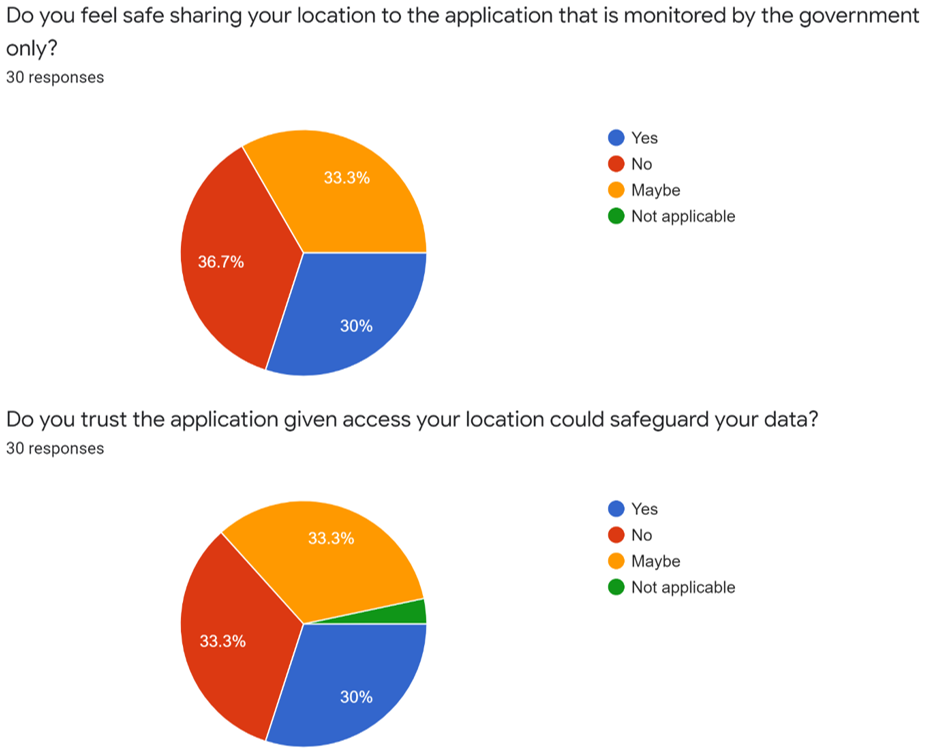
\includegraphics[width=14cm]{quantitative-01.png}
              \caption{}
              \label{fig:quantitative-01}
            \end{figure}
            \begin{figure}[H]
              \centering
              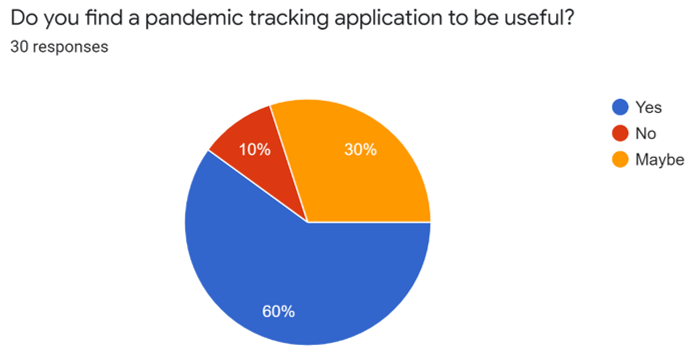
\includegraphics[width=12cm]{quantitative-02.png}
              \caption{}
              \label{fig:quantitative-02}
            \end{figure}
            \begin{figure}[H]
              \centering
              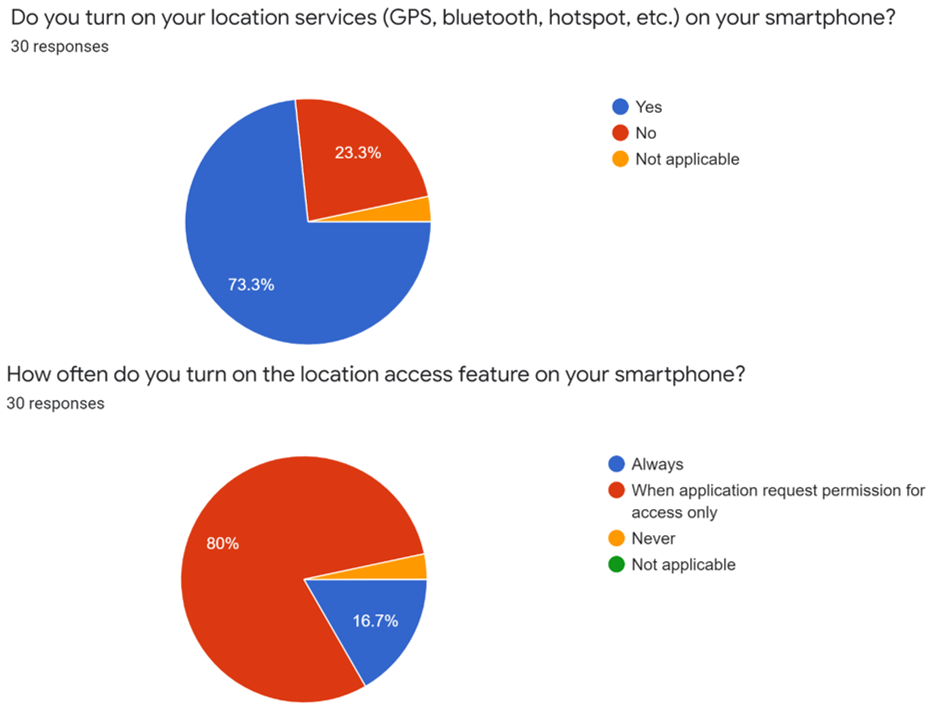
\includegraphics[width=14cm]{quantitative-03.png}
              \caption{}
              \label{fig:quantitative-03}
            \end{figure}

            \begin{itemize}
              \item Based on Figure \ref{fig:quantitative-01}, one-third of the respondents do not trust the data being protected regardless of it being a third-party or the government.
              \item Based on Figure \ref{fig:quantitative-02}, 60\% of the respondents thinks that a contact-tracing application would be useful.
              \item Based on Figure \ref{fig:quantitative-03}, approximately 73\% of the respondents turn on the location service feature which around 80\% gives location access only when the application request from the users.
            \end{itemize}
        \item \textbf{Interviews}
          \par Interview is a method of qualitative research. It is used as an approach for collecting descriptive opinions and views among different specific user categories. The interviewees were focused upon 3 different age groups consists of a primary school student, a retail worker, and a retired elderly that represents the age ranges of 0 to 17, 18 to 64, and above 65 respectively. The interview is composed of designed questions based on the evaluation from the survey, follow-up questions may also be included to gather more in-depth data. Thus, this helps to discover information based on their thinking, attitudes and even motivations. All interviewees have expressed consent to participate in this research study. The interviews were all conducted through online video call. The transcripts are attached below in Appendix \ref{appendix:qualitative}.
          \par \textbf{Findings}
            \begin{itemize}
              \item Minors do not think the application is necessary for them.
              \item Most adults are concern of the user privacy with location sharing.
              \item Includes accessibility features to accommodate elderly with disabilities.
            \end{itemize}
        \item \textbf{Insights}
          \begin{itemize}
            \item The number of application users could directly be influenced with the habit of users utilizing the location services or not, as it is necessary for the application to use the location services feature.
            \item Most participants do not trust the application to always collecting their location data.
            \item Most participants are doubtful of the government credibility in protecting their data. 
            \item Parental guidance and control could be a reason for minors not finding the application useful.
            \item Increasing accessibility features for accommodating user groups with disability could create a higher acceptance among the community.
            \item Proper digital privacy establishment is necessary for users to trust the application provider in handling their data.
          \end{itemize}
      \end{enumerate}

  \subsection{Sketches}
  \begin{figure}[H]
    \centering
    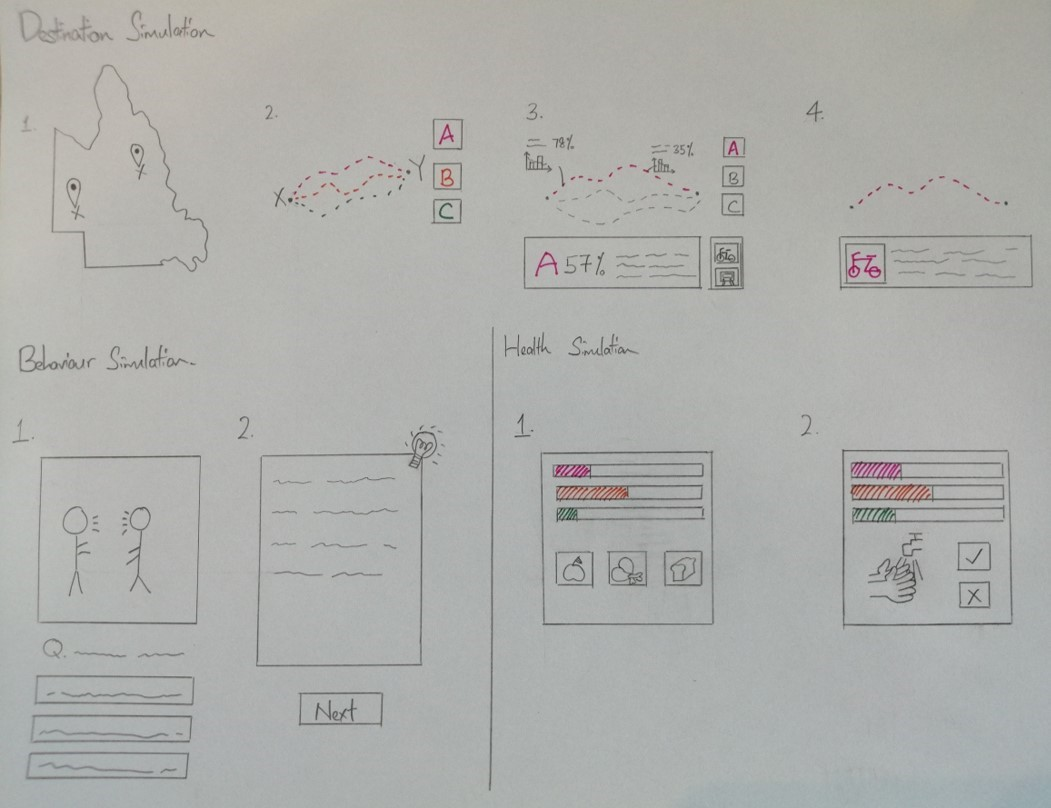
\includegraphics[width=18cm]{simulation.jpg}
    \caption{Simulation Sketches}
    \label{fig:simulation}
  \end{figure}
  \par Based on Figure \ref{fig:simulation}, various simulation ideas will be considered in further iterations as an implementation for the proposed solution. This provides a learning opportunity for the users, which creates interaction to achieve one of the product goals to make the platform to be more educational. Moreover, this would increase the user flow while the user interacting with the simulation, which creates possibility of more user scenarios in a simulated environment with real-life aspects during pandemic outbreak. Moreover, it could provide a pleasant user experience when information is conveyed via gamification with audio and visual components. Moreover, users could understand the value the application is trying to convey. Hence, simulation could navigate user through a journey that is projected with real-word aspects for embedding and implicit impressions for turning into habits and practices. In other words, it encourages habit and behaviour change when appropriate information is conveyed in an interactive manner be instilled into users under these special circumstances.

  \subsection{Prototypes}
    \subsubsection{Constrained Prototyping}
      \par Business Model Canvas is a method for constrained prototyping. The aim of a business model canvas is to explicit the values of the product through aligning various key elements during design planning phase. It provides a clear information outline for creating wireframe elements. Furthermore, it helps to visualize the conceptual idea of delivering a minimum viable product (MVP) which could serve as the basic form for the prototype.

      \par The canvas shown below in Figure \ref{fig:bmc} defines the general scope with descriptive points within the key elements section.

      \begin{figure}[H]
        \centering
        % 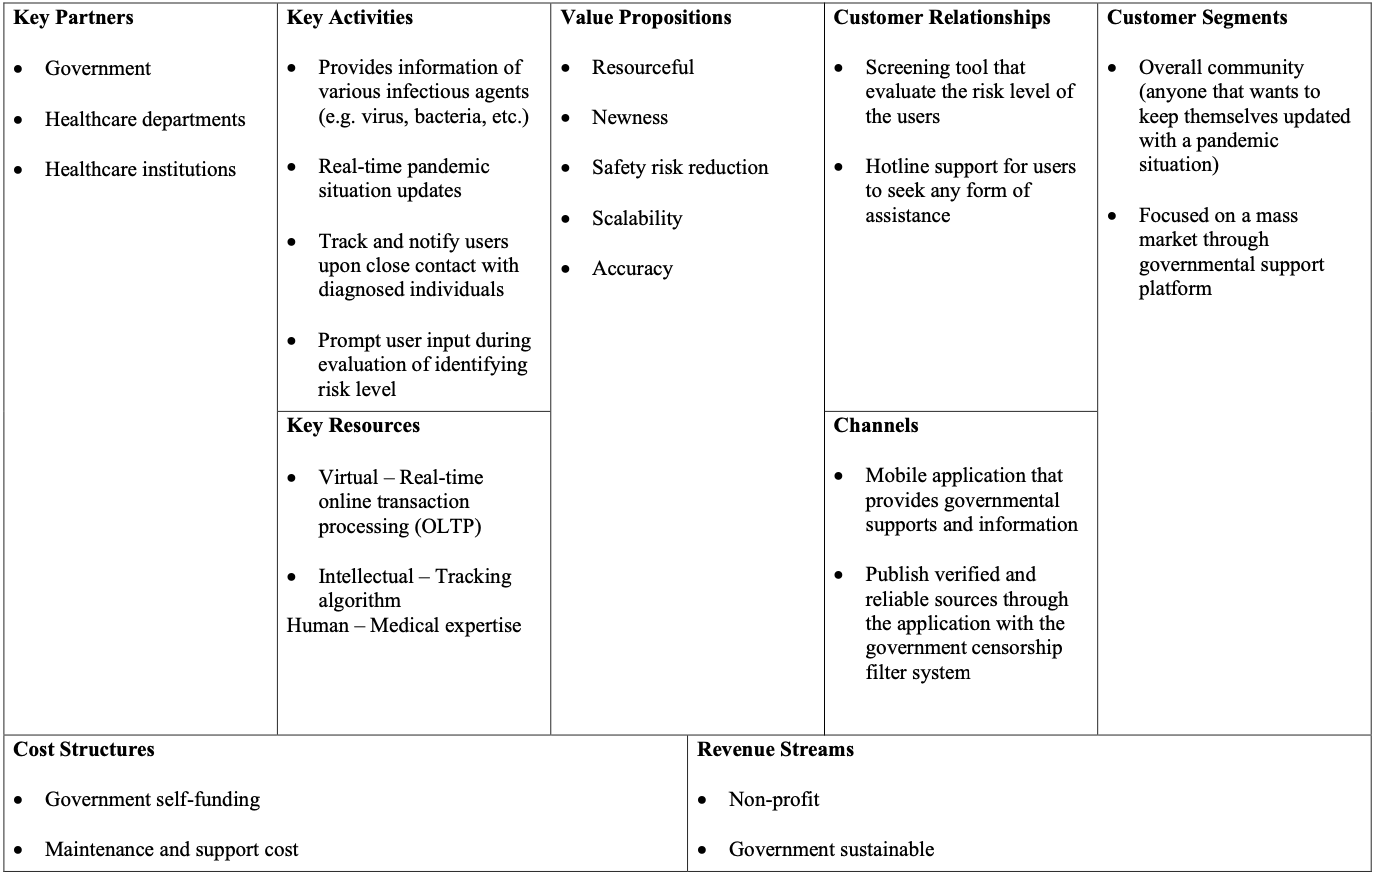
\includegraphics[width=21cm,angle=90,origin=c]{img/bmc.png}
        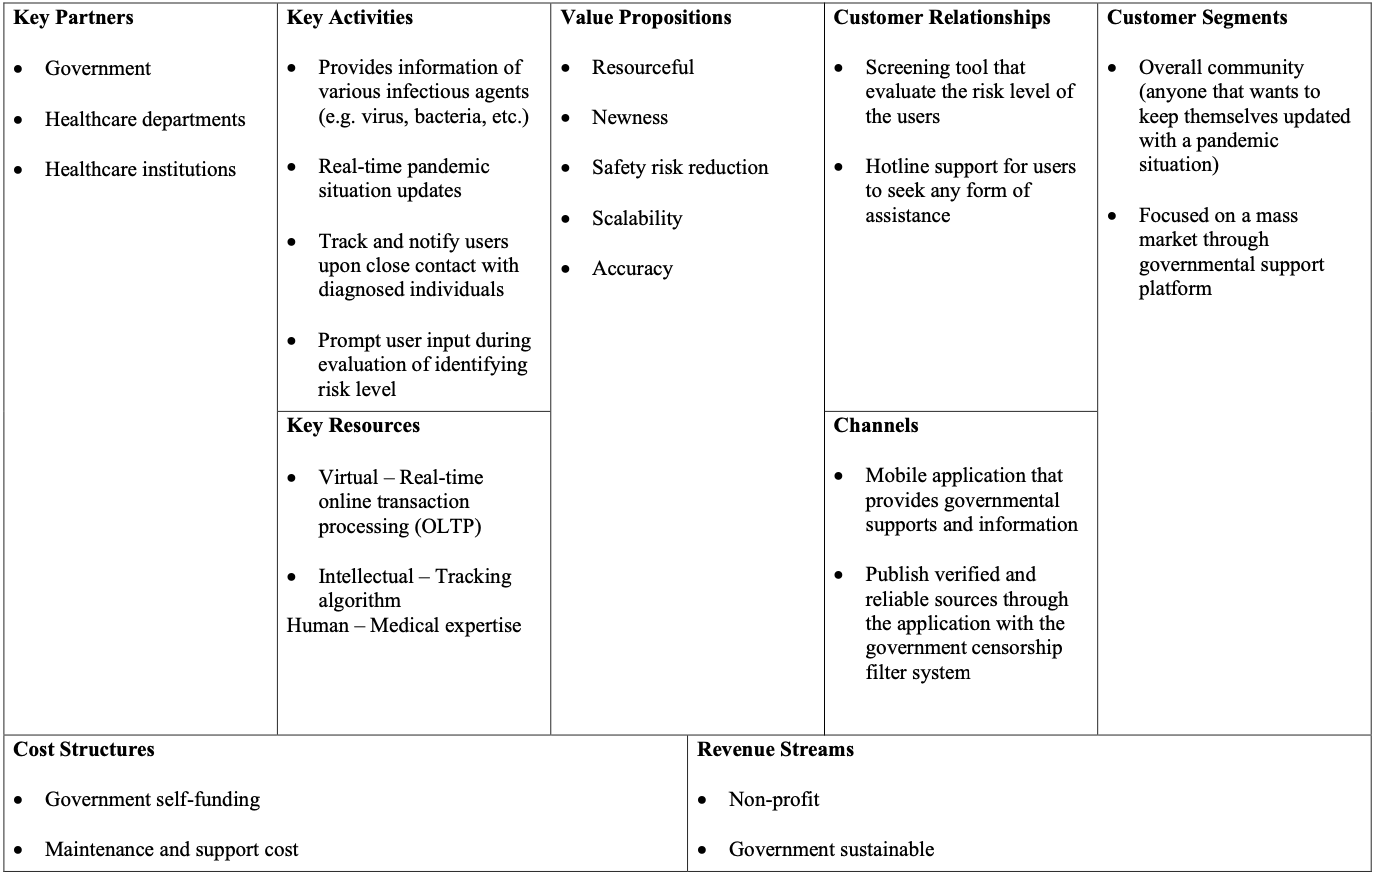
\includegraphics[width=18cm]{img/bmc.png}
        \caption{Business Model Canvas}
        \label{fig:bmc}
      \end{figure}
    
    \subsubsection{Paper prototyping}
      \par This approach is to provide a quick way to visualize the conceptual designs that could be a wireframe for the digital interfaces. A total of 9 simple interfaces of low-fidelity wireframes were created to showcase the general process of the possible solution.
      \begin{figure}[H]
        \centering
        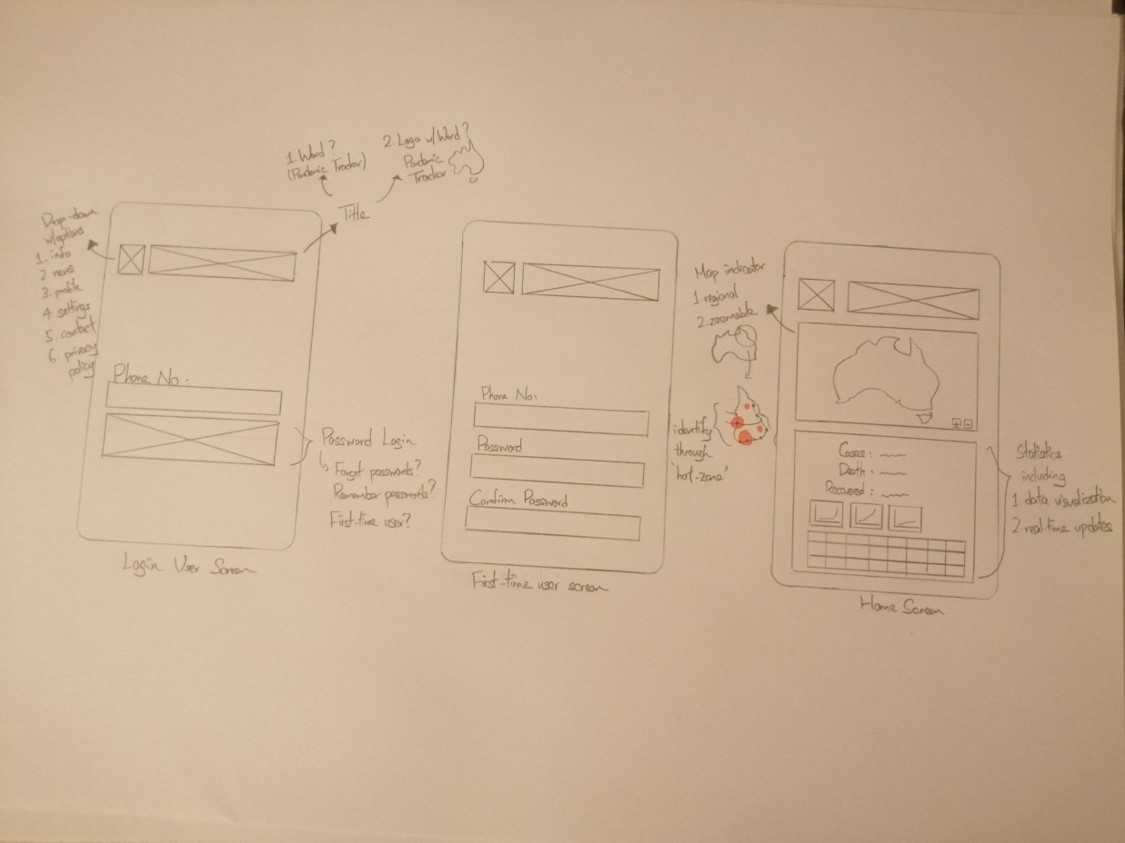
\includegraphics[width=18cm]{img/low-fidelity-prototype/sketch-1.png}
        \caption{Login, Register and Home Screen}
        \label{fig:prototype-01}
      \end{figure}
      
      \par Based on Figure \ref{fig:prototype-01}, the wireframe consists of the login, register and home screen interfaces, A valid phone number and a password is required for login. For first-time user, the login screen will have a link directing the user to the register screen to fill in the phone number and password to register as a member. Account recovery methods such as password reset will be included if the users forget their password. The home screen would include a heatmap indicator with statistical data of regional information including zone safety level, statistics, distribution of cases (orange dots in colour).
      
      \begin{figure}[H]
        \centering
        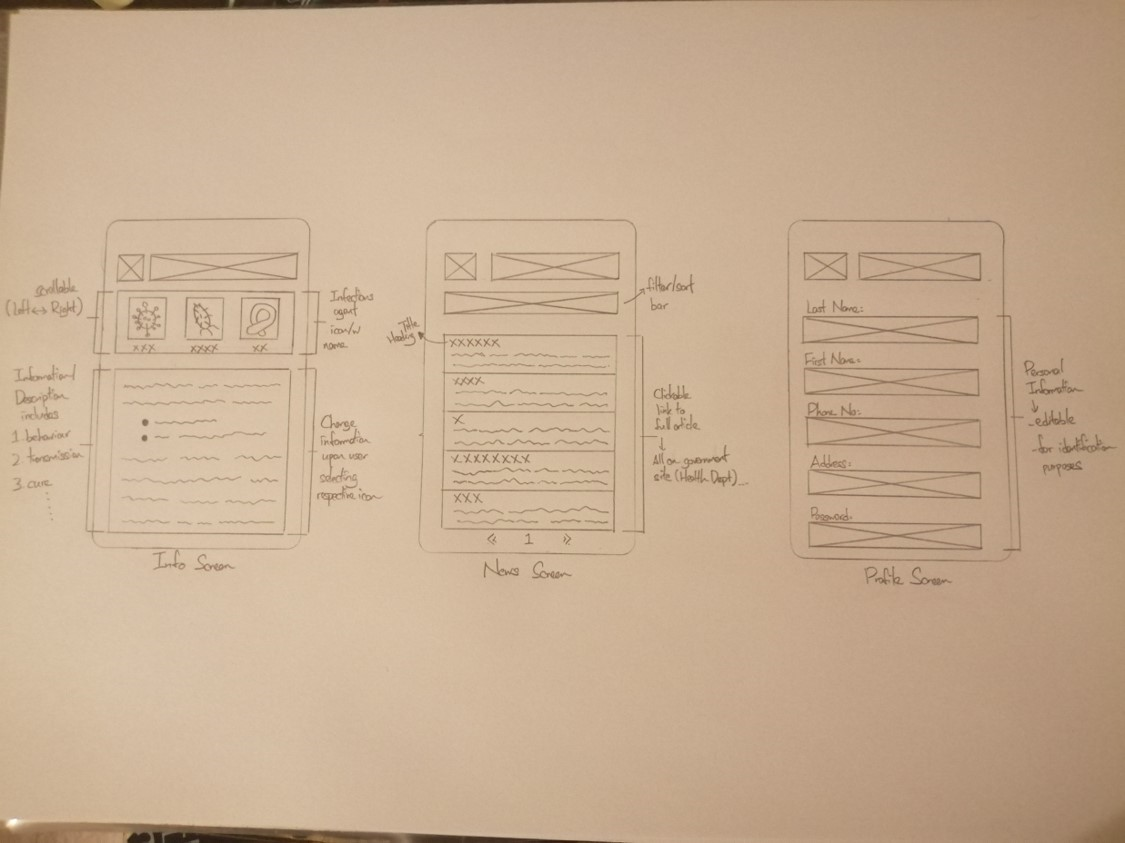
\includegraphics[width=18cm]{img/low-fidelity-prototype/sketch-2.png}
        \caption{Info, News and Profile Screen}
        \label{fig:prototype-02}
      \end{figure}

      \par Figure \ref{fig:prototype-02} shows the information, news and profile screen. Basic information of the infectious agents will be explained in layman terms which includes behaviour, characteristics, transmission and more. The following news screen are latest updated articles from verified publishers for any international and domestic news. The profile screen will display basic information consists of the authentic name of the user, phone no, and home address, which is crucial when immediate quarantine or government support is needed.

      \begin{figure}[H]
        \centering
        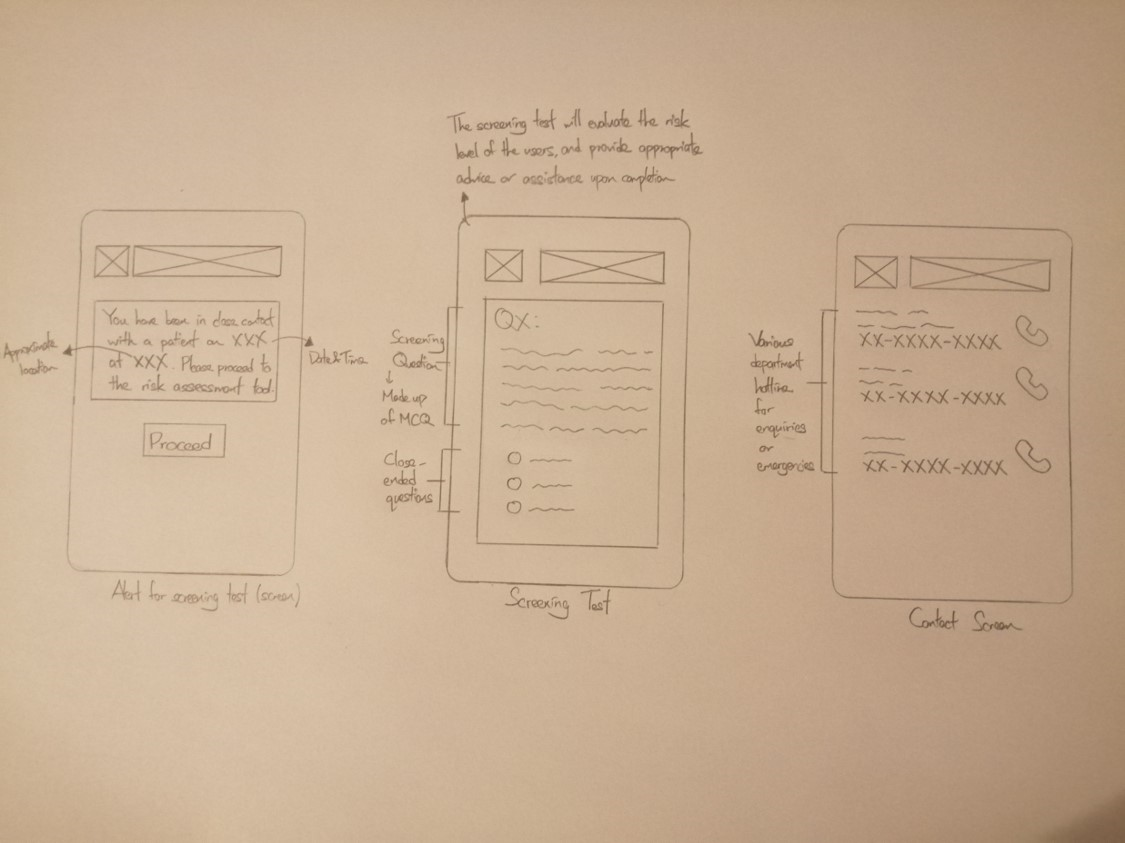
\includegraphics[width=18cm]{img/low-fidelity-prototype/sketch-3.png}
        \caption{Notification, Q\&A and Contact Screen}
        \label{fig:prototype-03}
      \end{figure}
      
      \par An alert notification, screening test and contact screen is shown in Figure \ref{fig:prototype-03}. The alert notification would pop up when the user has been verified having close contact with a diagnosed individual. The user will then be prompted to proceed to the Q\&A panel for a short evaluation. The result will display the user’s personal risk level, which may or may not necessarily to request medical support. Apart from this, the contact screen is listed with relevant government hotlines that could be helpful for enquiries or emergencies directly.

    \subsection{Further iterations}
      \subsubsection{Digital Prototyping}
        \par A high-fidelity sketch for multiple user interfaces will be created for interactive purposes. This approach would improve the data quality collected when users were asked to accomplish certain tasks and objectives. It increases the visual impact of the prototype making it more vivid with higher clarity, while delivering a higher quality prototyping to acquire a more accurate dataset.

      \subsubsection{Card Sorting}
        \par This process will be used to create feature segments to accommodate different interfaces being able to have high level of customization for low-fidelity prototype during usability testing. Its is advantageous to establish wireframes that delivers higher quality of the user requirements before advancing towards high-fidelity prototyping. Small customization for the same interface creates different versions of adaptions for usability testing which could collect more accurate and genuine perception from user feedbacks.

      \subsubsection{Usability Testing}
        \par Usability testing is set to be conducted starting from next iterations. The purpose is to evaluate a product through the prototype based on the feedbacks collected from users. It helps refining user requirement and visual design of the product through the prototype during testing. Moreover, it focused on how users interact with the prototype, completing the given tasks, and observe their behaviour during testing. It could collect valuable insights through learning the user’s behaviour and preference from the prototype. Thus, the insights could further improve the prototype for usability testing during each iteration.

      \subsubsection{Additional Features}
        \par Simulation and accessibility would be including in the next iteration.